\documentclass[10pt, letter]{article}

	\usepackage[margin=1in]{geometry}
	
	\usepackage[backend=bibtex, style=authoryear]{biblatex}
		
	\addbibresource{sources/sources.bib}
	\usepackage{hyperref}
	
			\title{\textsc{Neural Networks for Computed Tomography Imaging Spectroscopy of the Solar Atmosphere}}
			\date{\today}
			\author{Roy Smart \\ \url{roy.smart@montana.edu} \\ Montana State University, Department of Physics \\ Bozeman, MT 59717, USA}
			
	\usepackage{float}
	\usepackage{graphicx}
	\usepackage[font=scriptsize, labelfont=bf]{caption}
	\usepackage[font=scriptsize, labelfont=bf]{subcaption}


\begin{document}

	\maketitle
	
	\tableofcontents
	
	\begin{abstract}
		
		An important objective for future solar atmosphere observations is the advancement of snapshot imaging spectroscopy. Computed tomography imaging spectroscopy (CTIS) is a promising type of snapshot imaging spectroscopy that has seen applications in solar observations. Imaging spectroscopy using CTIS relies on the development of computed tomography algorithms to extract data from an instrument. Here, we propose to develop a computed tomography algorithm adapted to the environment of the solar atmosphere using neural networks. Success of such an algorithm will allow current and future CTIS missions to measure the dynamics of the solar atmosphere through the determination of line widths and doppler shifts.
		
	\end{abstract}
		
	\pagebreak
	
	\section{Problem Statement}
	
		
	
		\subsection{Background} \label{back_sec} 
		
			The solar transition region (TR) forms the boundary between the dense, cool plasma of the chromosphere and the chaotic environment of the million-degree corona. It is through this region that the plasma composing the solar atmosphere undergoes a rapid temperature increase, rising from 20,000 K to 1 MK over a distance of just tens of kilometers. The reasons behind this dramatic temperature rise and the mechanism through which the transition region influences the rest of the solar atmosphere have remained the subject of considerable debate (\cite{Innes2015}).
			
			The dynamic environment of the TR is demonstrated by the observation of so-called explosive events (EEs), discovered by \cite{Brueckner1983} using the \textit{High-Resolution Telescope and Spectrograph} (HRTS) and further investigated by \cite{dere1989} and \cite{Dere1994}. Explosive events are spectral features present in TR emission lines, which are defined by non-Gaussian line profiles showing Doppler shifts between 50--150 km/s (\cite{Brueckner1983}). These events have been shown to occur on spatial scales of 2'' -- 5'', last approximately 600s (\cite{dere1989}), and are consistent with a bi-directional flow through the TR (\cite{Dere1991}; \cite{Innes1997}).
			
			While the properties of explosive events have been well studied, investigators have been unable to reach a consensus on the cause of these events. It has been postulated that EEs are the signature of siphon flows within small-scale loops (\cite{Teriaca2004}), flows along spicules and macrospicules (\cite{Wilhelm2000}), plasma ejection and retraction (\cite{Huang2014}), and evidence of magnetic reconnection through the plasmoid instability (\cite{Innes2015}). Furthermore, EEs have been associated with other events in the solar atmosphere such as coronal microflares (\cite{Krucker2000}), reconnection in the photosphere (\cite{Tarbell1999}), and the chromospheric jets observed by \cite{DePontieu2011}.
			
			These competing views on the phenomena driving explosive events show that there is still much to be gained from further studies investigating explosive events. While revealing the phenomena driving these events remains an obvious goal, further study into explosive events should also aim to identify the origins of the energy that power explosive events, and the role of explosive events in the transportation of mass and energy through the solar atmosphere (\cite{Huang2014}).
			
			Measuring the properties of explosive events relies on imaging spectroscopy, a technique that aims to spectrally resolve each pixel of an image. Unfortunately, the capabilities of current imaging spectrographs may be inadequate for a thorough exploration of explosive events. This is because current imaging spectrographs (such as the Interface Region Imaging Spectrograph (IRIS)) can only view the sun through a thin slit, and must raster this slit across the sun to build up an image. This limited view prevents a complete characterization of explosive events, since only a small portion of the event can be observed at any one time.
			
			
			
			often associated with magnetic reconnection (\cite{Innes2015}).
			
			While the properties of explosive events have been well studied, the underlying physical phenomenon behind these events remains unknown. 
			
			
			Explosive events have been argued to have a spectral signature of siphon flows in small scale loops (\cite{Teriaca2004})
			
			
			There have been many proposed explanations for explosive events such as
			siphon flows in small-scale loops (\cite{Teriaca2004})
			
			Explanations offered by various parties to explain these events include: 
			
			There have many attempts to explain the spectral signal present in EEs.
			
			Over recent years, our understanding of the TR has evolved from a simple, 2D interface layer to a complex 3D volume rife with dynamic and unexplained phenomena. Explosive events are 
			
			Our understanding of TR has been steadily evolving from a simple, 2D interface layer to a complex, 3D volume
			
			Within the TR, we observe temperatures rising rapidly from 20,000K to 1 MK, but the reasons for this dramatic temperature increase and the mechanism through which this region heats the corona have remained the subject of considerable debate (\cite{Innes2015}). The TR was once 
			
			The dyna
			
			The complex dynamics of the TR is evidenced by the observation of so-called explosive events (EEs), discovered by \cite{Brueckner1983} using the \textit{High-Resolution Telescope and Spectrograph} (HRTS) and further investigated by \cite{dere1989} and \cite{Dere1994}. Explosive events are energetic phenomena present in TR emission lines that are characterized by non-Gaussian line profiles showing Doppler velocities between 50--150 km/s (\cite{Brueckner1983}). Attempts
			
			of non-Gaussian line-profiles displaying Doppler velocities of 50--150 km/s
			
			
			 and further investigated by \cite{dere1989} and \cite{Dere1994}. EEs are thought to be occurring continuously within the TR, and are characterized by non-Gaussian TR emission line profiles displaying a doppler shift of 50--150 km/s (\cite{Brueckner1983}).
			
			with a spatial size between 2'' to 5'' and a lifetime of about 600s (\cite{dere1989}).
			
			
			
			%%%%%%%%%%%%%%%%%%
		
			The solar physics community relies on a fleet of space-based instrumentation to study the solar atmosphere. Despite steady increases in both the spatial and spectral resolution of these instruments, the ability to completely track the transport of energy through this region has remained elusive (\cite{Innes2013}). Observations of the solar atmosphere have identified a wide range of energetic features that are thought to contribute to the heating of the solar atmosphere such as explosive events (\cite{Brueckner1983}, \cite{dere1989}, \cite{Dere1994}), coronal microflares (\cite{Krucker2000}), reconnection in the photosphere (\cite{Tarbell1999}), and the chromospheric jets observed by \cite{DePontieu2011}. Determining the mechanisms and the origin of the energy that drives these features has remained the subject of an ongoing debate which will most likely only be resolved through high-resolution \textit{snapshot imaging spectroscopy} (\cite{Innes2013}).
			
			Imaging spectroscopy describes the ability to spectrally resolve every pixel in an image of a scene (such as the Sun). Since a spectrally-resolved image can be represented by a 3D volume, data acquired through imaging spectroscopy is usually presented as a 3D datacube, known here as a \textit{spatial-spectral cube} SSC. Current instruments, such as the Interface Region Imaging Spectrograph (IRIS) (\cite{De Pontieu2014}), are designed for imaging spectroscopy of the solar atmosphere. These instuments build a spectrally-resolved image by scanning a slit across some field of view, building an SSC through rastering. Unfortunately, the SSC rendered using this technique is not cotemporal, i.e. each slice of the SSC was observed at a different time. Consequently, the SSCs observed by IRIS may be 
			
			Snapshot imaging spectroscopy (also known as snapshot hyperspectral imaging or simultaneous spectroscopic imaging) is a type of observation in which the spectrum for every pixel in a scene is acquired in a single ``snapshot'', i.e. with no scanning. This type of observation is in contrast to the imaging spectroscopy performed by spectrographs, such as the Interface Region Imaging Spectrograph (IRIS) (\cite{De Pontieu2014}) which must scan a slit across a scene (such as the Sun) to yield a spectrally resolved image. 
			
			Spectrally resolving an image in a single snapshot is ideal for observing dynamic objects such as the Sun, because it allows an unambiguous interpretation of the complex interrelationships between the multiple features observed in the solar atmosphere. Scanning imaging spectrographs such as the Interface Region Imaging Spectrograph (IRIS) (\cite{De Pontieu2014}) are also a
			
			Understanding the solar features
			
			Observation of the solar atmosphere presents a unique challenge for instrumentation design. 
			
			
			Investigations into the structure of the solar atmosphere, such as those discussed in the previous paragraph, have fueled steady advances in the spatial, spectral, and temporal resolution of solar observatories.
			
			
			the need for ever increasing spatial, spectral, and temporal resolution.  
			
			huge range of spatial, spectral and temporal features observed within. There is no known instrument design
			
			Current solar observatories may prove to be insufficient tools to fully characterize the features described above.  and current instrumentation lacks the ability to measure 
			
			Resolving this debate using the current generation of solar observatories such as narrow-band telescopes like the Atmospheric Imaging Assembly (AIA) on board the Solar Dynamics Observatory (\cite{aia}) and scanning imaging spectrographs like the Interface Region Imaging Spectrograph (IRIS) (\cite{De Pontieu2014}) can be difficult due to the complex spatial, spectral, and temporal nature of the solar atmosphere. Narrow-band telescopes are able to achieve a wide field at high temporal resolution at the expense of spectral resolution, while scanning spectrographs are able to achieve high spectral resolution but are forced to compromise between spatial and temporal resolution. While there is much we can learn from solar observations using these instruments, a more complete picture of the solar atmosphere requires the ability to observe the spatial, spectral and temporal structure of the Sun with increasingly high resolution.
			
			This 
			
			Current observational techniques such as narrow-band telescopes such as the Atmospheric Imaging Assembly (AIA) on board the Solar Dynamics Observatory (\cite{aia}) and conventional spectrographs like the Interface Region Imaging Spectrograph (IRIS) (\cite{De Pontieu2014}) can only go so far in resolving this mystery. To reach a consensus about these events it is likely we will need to conduct high-resolution, simultaneous spectroscopic imaging over the entire solar atmosphere. Simultaneous spectroscopic imaging, (also known as snapshot imaging spectroscopy, or snapshot hyperspectral imaging) is a type of observation in which the spectrum for every pixel in a scene is acquired in a single ``snapshot'', i.e. with no scanning. Spectrally resolving an image in a single snapshot is ideal for observing dynamic objects such as the Sun, because it allows an unambiguous interpretation of the complex interrelationships between the multiple features observed in the solar atmosphere.
			
			There has been a variety of instruments designed to achieve snapshot imaging spectroscopy over the past century. One technique in particular, known as computed tomography imaging spectroscopy (CTIS), has been successfully used to perform snapshot imaging spectroscopy in a variety of scientific fields, including solar observations \cite{fox1}. CTIS is a technique that attacks the problem of snapshot imaging spectroscopy by disposing of the slit used in conventional spectroscopy. Using this configuration, along with a 2D diffraction grating, allows a multitude of images to be formed at various diffraction orders and dispersion angles. In these images, the lack of a slit has allowed the spatial and spectral information to be multiplexed together, and CTIS relies on computational techniques to invert the multiplexing operation to recover a spectrally resolved image.
				
			 
		\subsection{Inversion}
			\label{inv_sec}
		
			
		
			Since a spectrally-resolved image can be represented by a 3D volume, we will refer to this sort of image as a spatial-spectral cube (SSC).  Computing this spatial spectral cube using images formed at multiple diffraction orders can be interpreted as a classic 3D tomography problem where $N$ projections are taken through a translucent 3D object in $x$, $y$ and $\lambda$ space (\cite{Bulygin:05}).
			\begin{figure}[h!]
				\centering
				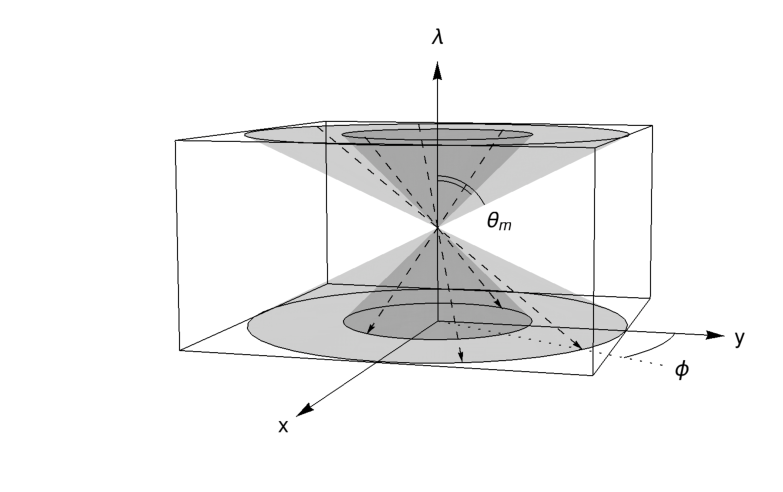
\includegraphics[width=0.5\textwidth]{figures/tomography}
				\caption{Geometry of the inversion problem for CTIS interpreted as a 3D tomography problem. $\theta_m$ describes the angle of the tomographic projection at each diffraction order and takes on discrete values, visualized by the nested cones. $\phi$ describes the dispersion direction and accepts continuous values. The four dotted lines are examples of particular projections through the spatial-spectal cube. Figure adapted from \cite{Bulygin:05}}
				\label{tomography}
			\end{figure}
			
			Using this representation, we can write the intensity in each order, $I_m$, of an object $v(x,y,\lambda)$ viewed by a CTIS in terms of the intergral equation provided by \cite{fox1}
			\begin{equation}
				I_m (x',y') = \int_B v(x' - \lambda \tan \theta_m \cos \phi, \; y' - \lambda \tan \theta_m \sin \phi, \; \lambda) \; d\lambda,
				\label{tomo_eqn}
			\end{equation}
			where $x'$ and $y'$ are image coordinates and $B$ is the passband of the instrument. Equation \ref{tomo_eqn} is a Fredholm integral equation of the first kind (\cite{RHB}) with a projection kernel. Our goal is then to invert Equation \ref{tomo_eqn} to recover the object $v(x,y,\lambda)$. This problem will be referred to as the ``inversion problem'' or just simply an ``inversion'' for the remainder of this proposal.
			
			The CTISs developed by Charles Kankelborg and his research group only take between $N=3$ and $N=6$ projections through the spatial-spectral cube. This limited number of projections does not provide enough information to completely reconstruct the SSC, i.e. in the case of the CTISs discussed below (MOSES and ESIS), inverting Equation \ref{tomo_eqn} is an \textit{ill-posed problem} (\cite{inversion}). This means that there are multiple solutions to the inversion problem that satisfy a particular set of projections. To uniquely solve the inversion problem a CTIS inversion algorithm (CIA) must find a way to eliminate incorrect solutions to the inversion problem. We can show that many of the solutions to the inversion problem are unphysical, that is, they are inconsistent with physical law and previous solar observations.
			
			Therefore, an inversion algorithm must use physical constraints to trim possible solutions to the inversion problem and accurately reconstruct the spatial-spectral cube (\cite{inversion}). In Section \ref{pwork} we will briefly explore advantages and disadvantages of the physical constraints used by current inversion algorithms, and in Section \ref{prop_sol} we will propose to use machine learning algorithms to approximate these physical constraints and solve the inversion problem.
			
		\subsection{Current and Planned CTISs}

			In the sections below, we will conduct a limited overview of the current and planned CTISs designed and built by Charles Kankelborg and his research group. A brief understanding of the optical system of each instrument will be helpful to understanding the goals of this proposal. 

			Each of the instuments in the succeeding sections is designed to fly on a Black Brant IX sounding rocket launched from White Sands Missile Range. Additionally, each instrument is constructed with a narrow passband in EUV which aims to alleviate intractability of the inversion process.

			\subsubsection{MOSES} \label{moses_intro}

				The Multi-Order Solar EUV Spectrograph (MOSES) has successfully undertaken two flights. The first flight occurred in 2005 and observed the Sun in He \textsc{ii} 304 \AA (\cite{fox1}) while the second flight was just recently completed in 2015 and observed the Sun in He \textsc{vii} 465 \AA (\cite{smart1}). 			
				 		
				\begin{figure}[h!]
					\centering
					\begin{subfigure}[t]{0.49\textwidth}
						\centering
						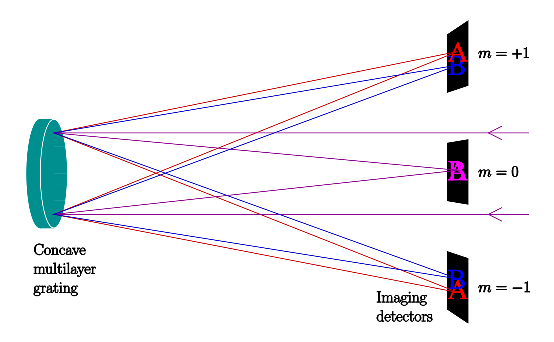
\includegraphics[height=2in]{figures/concave}
						\caption{Sketch of the optical system of MOSES}
						\label{optics}
					\end{subfigure}	
					~
					\begin{subfigure}[t]{0.49\textwidth}
						\centering
						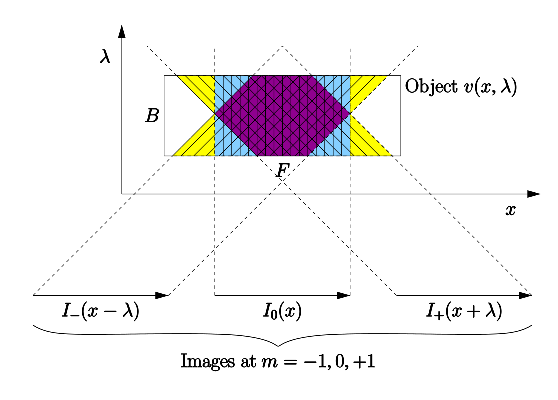
\includegraphics[height=2in]{figures/moses_cube}
						\caption{The analogue of Figure \ref{tomography} for the MOSES instrument.}
						\label{moses_tomo}
					\end{subfigure}	
					\caption{Two diagrams used to visualize the imaging system of the MOSES instrument. Figure \ref{optics} demonstrates how a bimodal spectral signal represented by a red `A' and a blue `B' are imaged by the MOSES optical system. Figure \ref{moses_tomo} imagines the MOSES optical system as a 2D tomographic projection through a spatial-spectral cube. Figures courtesy of \cite{fox1}}
				\end{figure}
				MOSES is a CTIS that uses a single concave diffraction grating to produce images in three spectral orders, $m=-1,0,1$, as in Figure \ref{optics} (\cite{kankel1}).
				Since the diffraction grating of MOSES has rulings along only one direction, the dispersion is only in one direction. In the parlance of Figure \ref{tomography}, $\phi$ is restricted to the values of 0 and $\pi$ and then, without loss of generality, we can represent the 3D projections of Figure \ref{tomography} as 2D projections through a plane, as in Figure \ref{moses_tomo}.
				
				MOSES presents several challenges against achieving an accurate inversion. The most prevalent of these is the large, unknown point-spread function (PSF) of the instrument. The scale of this PSF is a compromise that allows MOSES to form images in three diffraction orders from a single optic (\cite{kankel1}).

			\subsubsection{ESIS} \label{esis_intro}
			
				The EUV Snapshot Imaging Spectrograph (ESIS) is the next generation of a CTIS developed by Kankelborg and his research group. This instrument will be equipped with one large focusing primary mirror, and small, dedicated diffraction gratings for each detector. The first flight is planned for 2019 and the instrument will be equipped with four detectors to image the $m=1$ order in four separate dispersion directions. After the first flight has been completed, the system will undergo upgrades to install two additional gratings and detectors for a total of six tomographic projections. 
				
				The tomographic projections of the ESIS instrument can be visualized in terms of Figure 1. The dedicated diffraction gratings are arranged in an octagonal pattern, producing projections at $\phi = 0$, $\pi/8$, $\pi/4$, $3 \pi / 8$, $\pi /2$, $5 \pi /8$, and $3 \pi /4$. Since these projections are not all in the same plane (unlike the MOSES arrangement), the inversion problem cannot be reduced to two dimensions and must be solved in 3D.
			
		\subsection{Related Work} \label{pwork}
			
			The task of inverting MOSES data has already been undertaken by several research projects (\cite{inversion}, \cite{fox1}). The most effective inversion algorithm developed by these efforts is known as the \textit{smooth multiplicative algebraic reconstruction technique} (SMART) developed by \cite{kankel2} based off of earlier algebraic reconstruction techniques invented by \cite{Gordon70} and refined by \cite{Okamoto:91}. As discussed in Section \ref{inv_sec}, any CTIS inversion algorithm must use physical constraints to make the problem tractable. In the case of SMART, it uses the property that its solutions to the inversion problem must satisfy positivity, since intensity is a positive quantity (\cite{kankel2}).
			
			The result is a very efficient algorithm that has been successfully used to determine doppler shifts and line profiles of explosive events in He \textsc{ii} (\cite{rust1}).
			Unfortunately, it has proven difficult to convince SMART to produce physical inversions across the entire MOSES dataset. This unphysicality is mainly produced by an artifacts known colloquially as \textit{plaid}. As an example, in Figure \ref{plaid} we can see that the bright object in the center has been blurred at the angles: $\theta=-\pi/4$, 0, and $\pi/4$ (with respect to the vertical) resulting in plaid. Such structures are considered to be unphysical since intensity is usually concentrated along horizontal spectral lines and not at angles of $\pi/4$.
			\begin{figure}[h!]
				\centering
				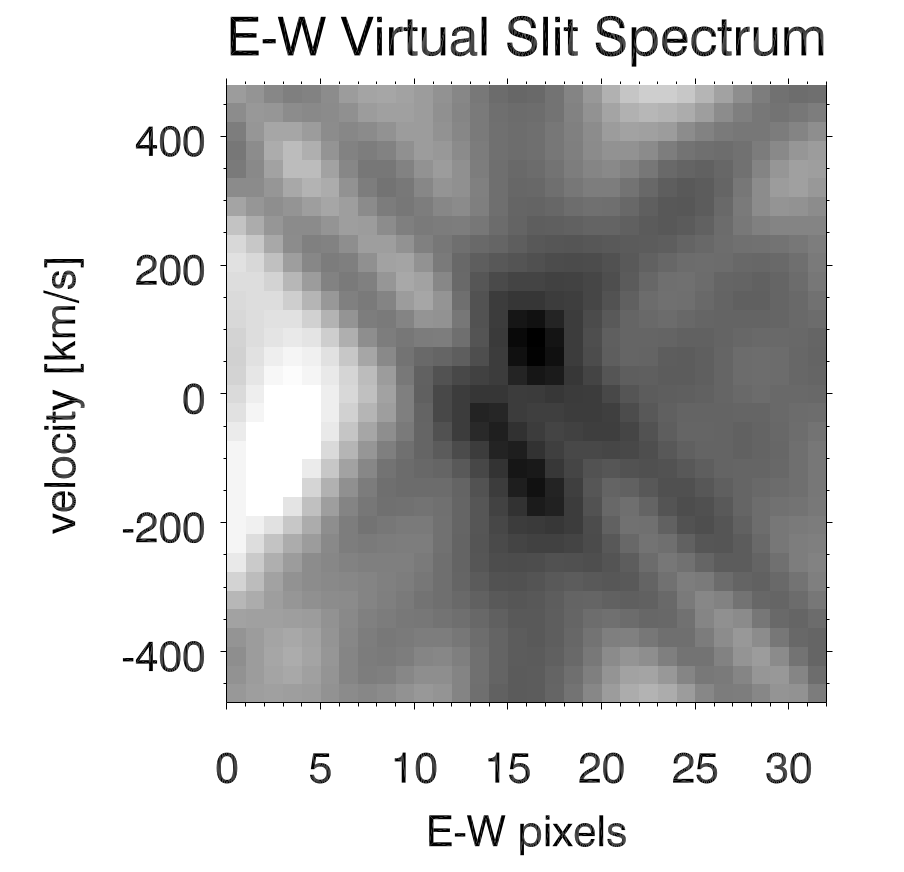
\includegraphics[width=0.3\textwidth]{figures/plaid}
				\caption{An example of plaid produced by SMART. The vertical dimension is the spectral dimension in units of relative doppler shift from line center, and the horizontal axis is position measured in pixels. Image courtesy of Thomas Rust.}
				\label{plaid}
			\end{figure}
			
			Plaid occurs whenever SMART attempts to invert a set of CTIS images with a background signal. Therefore, to yield plausible results using SMART, the background must be manually subtracted to isolate and successfully invert the area of interest. This operation prevents the creation of an automated, global inversion process for MOSES data.

		\subsection{Project Goals}
		
			Using the performance of SMART as a baseline, I would like to develop a more robust algorithm to perform inversions of data produced by a CTIS such as MOSES and ESIS. The specific goals of my algorithm are to produce inversions with minimal to no plaid artifacts while maintaining an execution time competetive with SMART. I will then use this algorithm to complete my ultimate goal of computing an inversion over the entire MOSES dataset, and later on ESIS after the instrument has been completed and launched.
		
	\section{Proposed Solution} \label{prop_sol}
	
		So far, all CIAs have utilized physical constraints derived from first principles (such as positivity). This is not the only way however, instead an inversion algorithm could build physicality constraints based off of direct observation of the solar spectrum. For example, IRIS has been measuring the spectrum of the Sun since 2013 (\cite{De Pontieu2014}), and has amassed a large dataset composed of observations of the solar spectrum. An inversion algorithm that incorporates these observations has the potential to calculate inversions with greater accuracy because it would have the capability to eliminate solutions to the inversion problem that are inconsistent with the observations provided by IRIS.
		
		One possible way to appy a set of solar spectroscopic observations to an algorithm is by using machine learning. Machine learning is a problem solving technique that allows a computer to learn a relationship between a set of problems and their associated solutions. Artificial Neural Networks (ANNs) are possibly the most popular type of machine learning algorithms, and they have been used successfully to solve a wide variety of problems such as classification, function approximation, and data compression. Recently, it has been shown that ANNs have the capability to solve problems critical to solar data analysis such as denoising (\cite{DAEC}) and PSF deconvolution (\cite{nn_psf}). ANNs have even been successful in solving ill-posed problems (\cite{Kruglov2013}), inversion problems (\cite{Jafarian2015}) and computed tomography problems (\cite{Boublil2015}). Due to the success of ANNs at solving these types of problems I hypothesize that a CIA represented by a neural network and trained using real solar spectroscopic data would be able to form reasonable solutions to the inversion problem.
		
		\subsection{A Brief Introduction to Neural Networks}
			
			Neural networks are built using computational units known as neurons. A neuron is . A neural network is built by arranging some number of neurons into layers (Figure \ref{ann_fig}). The first layer is the input layer and it represents the input to the network. Similarly, the last layer is the output layer and represents the output of the network. The neurons between these layers are grouped into so called \textit{hidden layers} and provide the computational power of the network. In this architecture, every neuron in each layer (except the output layer) is connected to every other neuron in the succeeding layer. These connections are weighted, and the weights are learned by the network during training.
			
			\begin{figure}[h!]
				\centering
				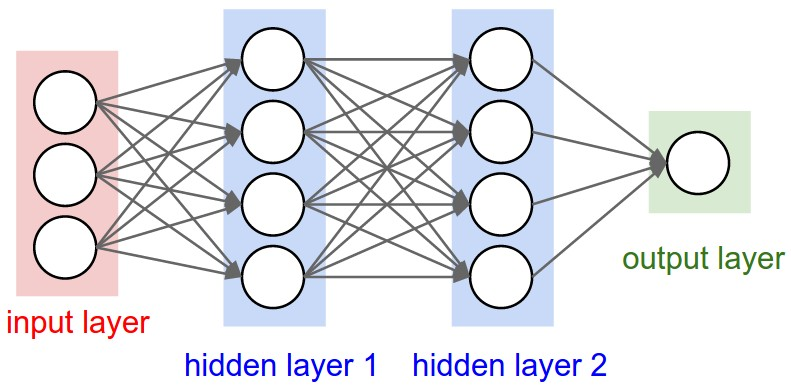
\includegraphics[width=0.4\textwidth]{figures/ann2}
				\caption{Diagram of a simple ANN with two hidden layers with four neurons each.}
				\label{ann_fig}
			\end{figure}
			
			A large \textit{training set} of example problems with known solutions is used to train the neural network. These problems are fed into the neural network which is then penalized according to the error between the neural network's answer and the accepted answer. Based off of this feedback, the neural network adjusts its weights to minimize the error. The most common algorithm used to train a neural network in this fashion is known as back-propagation, which uses the method of gradient descent to minimize the error (\cite{ai}).
		
		\subsection{Inversion Using Neural Networks}
		
			With the basic description provided in the previous section, we can begin to discuss how we one would build a CIA using neural networks, which we will call a \textit{CTIS inversion neural network} (CINN). To summarize Section \ref{inv_sec}, a CIA solves a computed tomography problem, which reconstructs a 3D object using a set of 2D projections. Thus, a CINN's input layer will be a set of neurons representing each pixel in each 2D projection and a CINN's output layer will be a set of neurons representing each voxel of the SSC. These layers will be connected by an unknown number neurons to be determined during training. 
					
			To create the training dataset, we start by constructing a spatial-spectral model of the Sun. Since MOSES and ESIS are designed with a narrow passband, the spectral range of this model need not be immense, but it should be representative of the Sun as observed by MOSES and ESIS. As indicated above, this model will be composed of direct spectroscopic observations of the Sun from existing instruments. However, there are no spectrographs that observe the Sun in the same passband as ESIS and MOSES, so we will use observations of emission lines with comparable formation temperatures to that of the emission lines in the passband of MOSES and ESIS. 
			
			This spatial-spectral model forms what we will call the ``truth dataset''. From the truth dataset, we will generate the ``input dataset'' by using a forward model of the optical system of each instrument. MOSES and ESIS have different optical systems, so to solve the inversion problem for each instrument, we will be required to train two neural networks. The input and truth datasets taken together form the training dataset. During training, data from the input set will be fed into the CINN, and data from the truth dataset will be compared to the output of the CINN to direct the learning process.
			
			\subsubsection{MOSES Inversion} \label{moses_inv}
			
				In Section \ref{moses_intro} we discussed how the inversion problem for MOSES can be reduced from a 3D to a 2D computed tomography problem. This dimensionality reduction is fortunate, because the dimensionality of the truth dataset, input dataset and the CINN itself may all be reduced accordingly. Therefore, a MOSES CINN leveraging this dimensionality reduction can only reconstruct a slice of the SSC, and must be scanned across a MOSES image to reconstruct the entire SSC.
				
				To build the truth dataset for a MOSES CINN, we simply acquire an array of SSC slices, such as those produced by traditional spectrographs. Using the observations produced by IRIS to construct the truth dataset is an obvious choice. This is because the images are easily accessible, the dataset is sufficiently large, and the Si \textsc{iv} line observed by IRIS has a comparable formation temperature to the He \textsc{ii} line captured by MOSES (SOURCE???).
			
				The forward model of MOSES will be used to make the input dataset. This model will have four main components. First, the projections described by Figure \ref{moses_tomo} are applied to each SSC slice. Next, the projections will be convolved with an approximation of the MOSES PSF. Then, both the truth and input datasets are downsampled to match the spatial resolution of MOSES and the truth dataset is downsampled to match the spectral resolution of MOSES. Finally, we will apply shot noise to define the exposure length and readout noise consistent with the readout noise of the real instrument. This approach forms a realistic approximation to the MOSES system, which is critical to training the CINN to appropriately interpret the data from the real instrument.
			
			\subsubsection{ESIS Inversion}
			
				Unlike MOSES, recovering the SSC from ESIS data requires a 3D solution to the inversion problem (Section \ref{esis_intro}). Therefore, the truth dataset of an ESIS CINN takes the form of an array of SSCs, which are most easily acquired by using IRIS in raster mode. Unfortunately, few of the rasters produced by IRIS are taken at a high enough spatial resolution to provide a realistic SSCs, and we will need a large number of SSCs to effectively train a CINN. There are several approaches to circumventing this problem, the easiest of which is to naively stacking spectral images to form a psuedo-realistic SSC to be inserted into the truth dataset. 
				
				The forward model of ESIS will be similar to that of MOSES except that there are more projections which are taken at different angles through the SSC, and there is likely no need to apply a PSF since the PSF of ESIS is predicted to be smaller than a pixel.
		
		\subsection{Preliminary Results}
		
			To test if a CINN could be a useful inversion tool, we trained a CINN to invert a simplified forward model of MOSES. This CINN used a input dataset that did not incorporate elements of the MOSES forward model discussed in Section \ref{moses_inv} such as the PSF, shot noise or readout noise. While this simplification is certainly unrealistic, this CINN serves to illustrate a proof-of-concept and to justify additional research into this method.
			
			This CINN was trained using approximately 500k truth images with a size of $21 \times 21$ pixels. These images were extracted from the IRIS Si \textsc{iv} 1403 \AA{} dataset, and were background subtracted to further simplify the inversion problem for this test.
			
			This CINN was trained on an Nvidia 980 GPU using the Caffe (\cite{jia2014caffe}) neural network library. 
			
			\begin{figure}[h!]
				\centering
				\begin{subfigure}[t]{0.18\textwidth}
					\centering
					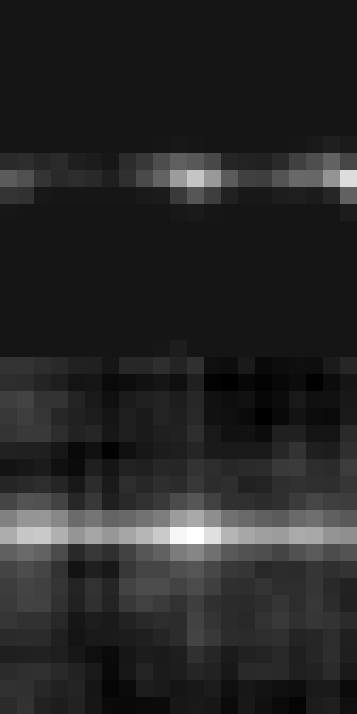
\includegraphics[width=\textwidth]{figures/inv1}
				\end{subfigure}	
				~
				\begin{subfigure}[t]{0.18\textwidth}
					\centering
					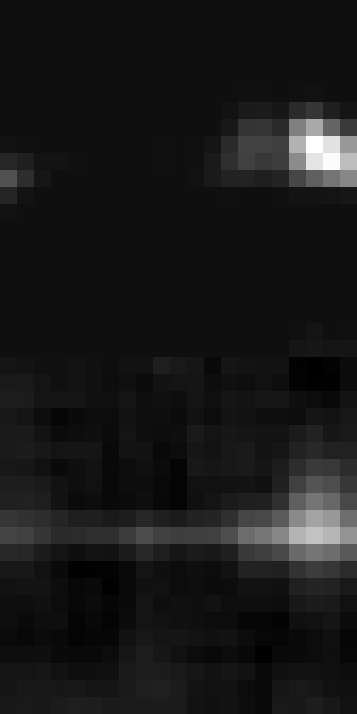
\includegraphics[width=\textwidth]{figures/inv2}
				\end{subfigure}	
				~
				\begin{subfigure}[t]{0.18\textwidth}
					\centering
					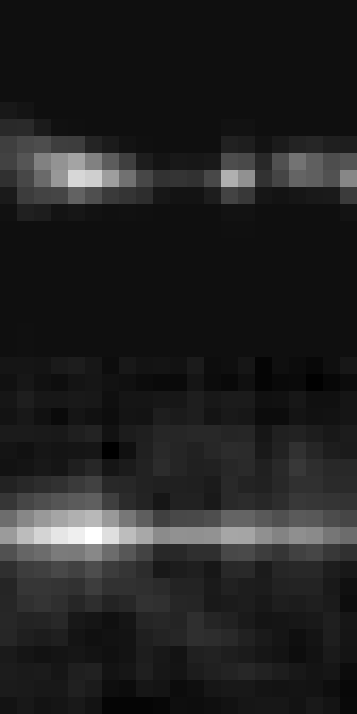
\includegraphics[width=\textwidth]{figures/inv3}
				\end{subfigure}	
				~
				\begin{subfigure}[t]{0.18\textwidth}
					\centering
					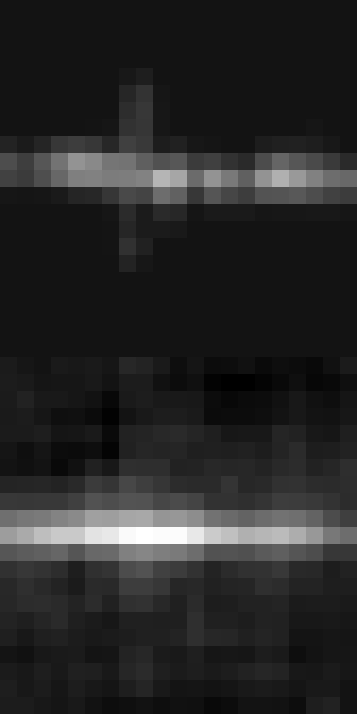
\includegraphics[width=\textwidth]{figures/inv4}
				\end{subfigure}	
				~
				\begin{subfigure}[t]{0.18\textwidth}
					\centering
					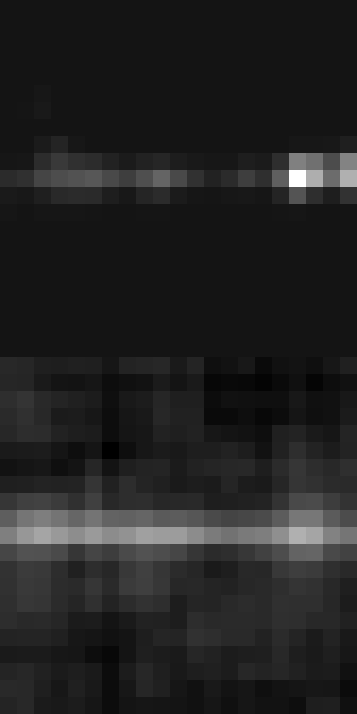
\includegraphics[width=\textwidth]{figures/inv5}
				\end{subfigure}	
				\caption{A visualization of the inversions produced by a simple implementation of a MOSES CINN. The top image is the truth image and the bottom images is the output of the CINN.}
			\end{figure}
			
			
		
	\section{Relevance to Heliophysics}
	
	\section{Project Timeline}
	

	\printbibliography

	
\end{document}

